\documentclass[final]{siamltex}

% for red MarginPars
\usepackage{color}

% for \boldsymbol
\usepackage{epsfig}

% total number of floats allowed on a page
\setcounter{totalnumber}{100}

% float page fractions
\renewcommand{\topfraction}{0.9}
\renewcommand{\bottomfraction}{0.9}
\renewcommand{\textfraction}{0.2}

% MarginPar
\setlength{\marginparwidth}{0.75in}
\newcommand{\MarginPar}[1]{\marginpar{\vskip-\baselineskip\raggedright\tiny\sffamily\hrule\smallskip{\color{red}#1}\par\smallskip\hrule}}

% for non-stacked fractions
\newcommand{\sfrac}[2]{\mathchoice
  {\kern0em\raise.5ex\hbox{\the\scriptfont0 #1}\kern-.15em/
   \kern-.15em\lower.25ex\hbox{\the\scriptfont0 #2}}
  {\kern0em\raise.5ex\hbox{\the\scriptfont0 #1}\kern-.15em/
   \kern-.15em\lower.25ex\hbox{\the\scriptfont0 #2}}
  {\kern0em\raise.5ex\hbox{\the\scriptscriptfont0 #1}\kern-.2em/
   \kern-.15em\lower.25ex\hbox{\the\scriptscriptfont0 #2}}
  {#1\!/#2}}

\begin{document}

%==========================================================================
% Title
%==========================================================================
\title{User's Guide to Stochastic Diffusion/Reaction Code}

\maketitle

\section{Introduction}

\section{Source Code}
%%%%%%%%%%%%%%%%%%%%%%%%%%%%%%%%%%%%%
\begin{figure}[tb]
\centering
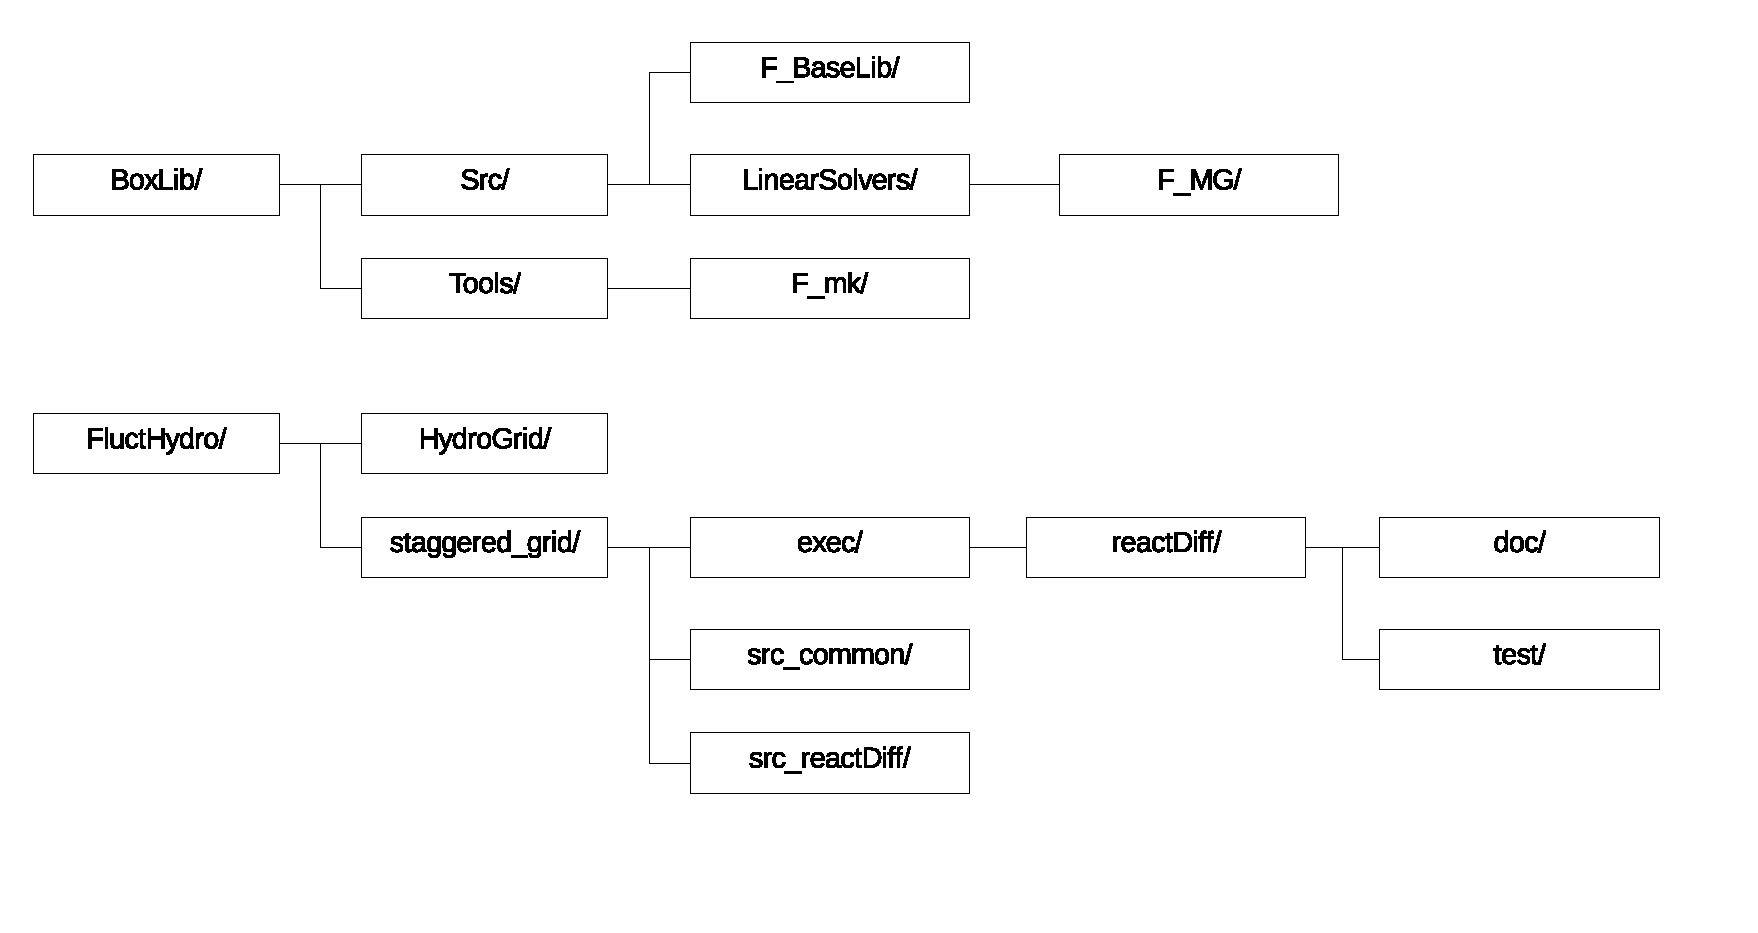
\includegraphics[width=6in]{./directory}
\caption{\label{fig:directory}Directory structure.}
\end{figure}
%%%%%%%%%%%%%%%%%%%%%%%%%%%%%%%%%%%%%
\begin{itemize}

\item {\tt BoxLib/}

\begin{itemize}

\item {\tt Src/}

\begin{itemize}

\item {\tt F\_BaseLib/}

Core libraries for parallelization of structured grid data.

\item {\tt LinearSolvers/F\_MG/}

Core libraries for linear solvers (for implicit diffusion) and diffusion stencils.

\end{itemize}
\end{itemize}

\begin{itemize}

\item {\tt Tools/F\_mk/}

Make system variables and flags.

\end{itemize}
\end{itemize}

\begin{itemize}

\item {\tt FluctHydro/}

\begin{itemize}

\item {\tt HydroGrid/}

\item {\tt staggered\_grid/}

\begin{itemize}

\item {\tt exec/reactDiff/doc/}

Contains the document you are reading right now!

\item {\tt exec/reactDiff/test/}

This is the compilation directory.  Contains a GNUmakefile and inputs files.

\item {\tt src\_common/}

Source code shared by all our staggered grid codes.  Contains generic namelist parameters
and routines for boundary conditions, divergence, etc.

\item {\tt src\_reactDiff/}

Source code specific to this reaction/diffusion problem.

\end{itemize}
\end{itemize}
\end{itemize}

\subsection{Compilation}
Go to {\tt FluctHydro/staggered\_grid/exec/reactDiff/test/} and edit the 
{\tt GNUmakefile} settings to your liking (below) and simply type {\tt 'make'}.\\
\begin{verbatim}
NDEBUG    :=           # 'not debug'.  use 't' for an optimized build
MPI       := t         # use 't' to build an mpi executable
OMP       :=           # use 't' to build an OpenMP threadded executable
PROF      :=           # use 't' to turn on code profiling
COMP      := gfortran  # fortran compiler
CCOMP     := gcc       # c compiler
MKVERBOSE := t         # make verbosity
\end{verbatim}

\subsection{Input Parameters}

\section{Equations}

\section{Operator Splitting}

\section{Diffusion}

\section{Reactions}

\end{document}
